\begin{figure*}
    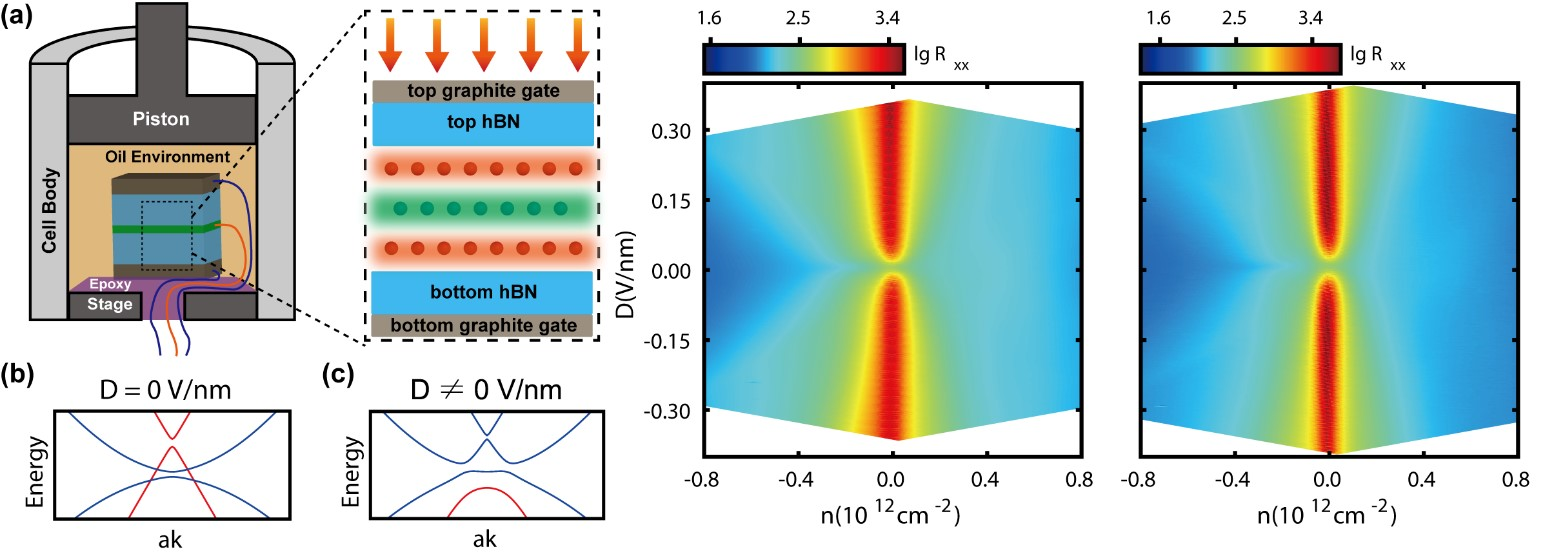
\includegraphics{figures/Figure_1.jpg}% Here is how to import EPS art
    \caption{\label{fig:1} Schematic of experimental setup and transport characterization.\\
    (a) Schematics of hydrostatic pressure setup. (b), (c) Schematics of How the displacement field influences the band structure of tri-layer ABA graphene.
    In the absence of displacement field D, the low energy bands include two monolayer-like bands with linear dispersion (red curve \& blue curve) 
    and two bilayer-like bands with parabolic dispersion (cyan curve \& green curve).
    When D is non-zero, these two bands hybridize, leading to a gap opening at the charge neutrality point, making the system insulate.
    (d), (e) device characterization before and after 1.0 GPa hydrostatic pressure by using the four-terminal longitudinal resistance $R_{xx}$ 
    as a function of carrier density $n(10^{12}cm^{-2})$ and displacement field D(V/nm). 
    Along the charge neutrality profile, the resistance increases dramatically as D increases, indicating a gap opening reflecting the device's good quality.
    }
\end{figure*}

\begin{figure*}
    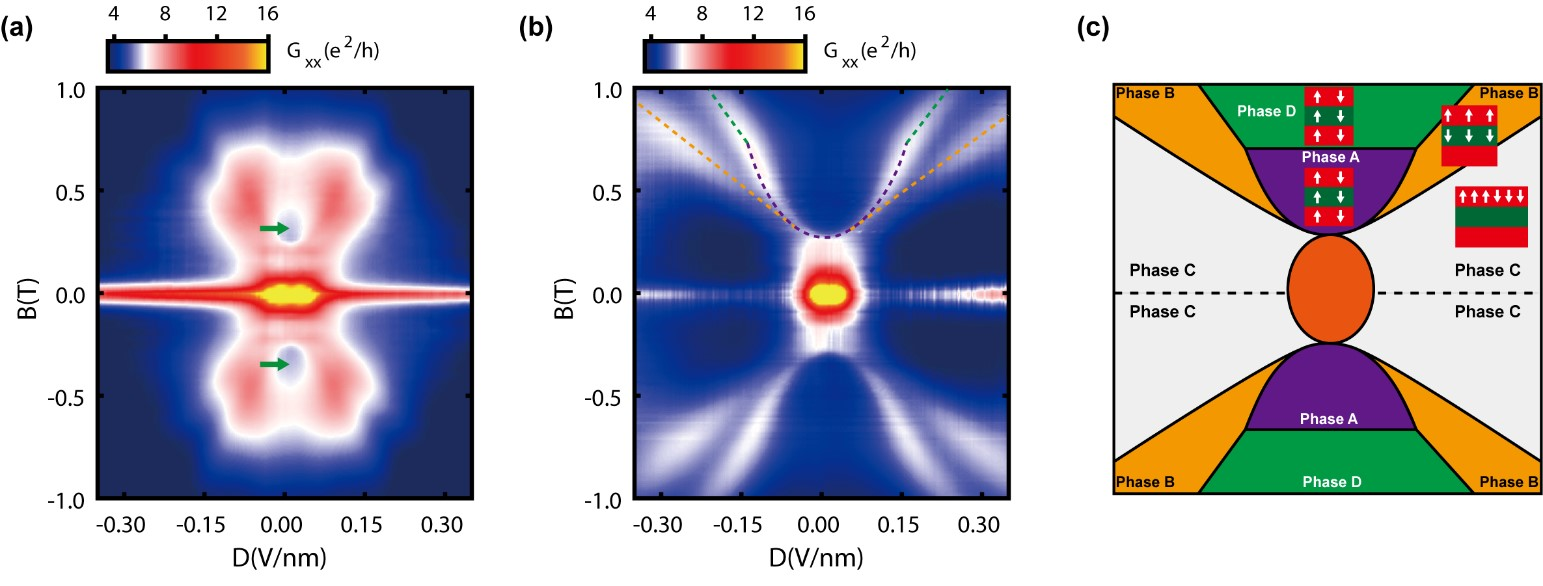
\includegraphics{figures/Figure_2.jpg}% Here is how to import EPS art
    \caption{\label{fig:2} Phase diagrams at the charge neutrality point before and after 1.0 GPa hydrostatic pressure.\\
    Here, Figures 2(a) and 2(b) show the phase diagrams of four-terminal longitudinal conductance $G_{xx}$ in unit of $\frac{e^2}{h}$ as a function of B(T) and D(V/nm), 
    with B ranges from -1.0 T to 1.0 T and D ranges from -0.30 V/nm to 0.30 V/nm, it is noted that the values larger than 16 has been rescaled to 16. 
    (a) shows the phase diagram at 0 GPa. A prominent feature emerges around D = 0 V/nm and B = 0.3T, indicated by the green arrow. 
    (b) the phase diagram at 1GPa shows visible traces of phase boundary (marked by dashed lines of different colours), 
    indicating first-order phase transitions between different ground states.
    This phase diagram is converted into a cartoon shown in (c). Different regions are filled with different colours, and specific phases are labelled with A, B, and C, 
    demonstrating the existence of different ground states.}
\end{figure*}

\begin{figure*}
    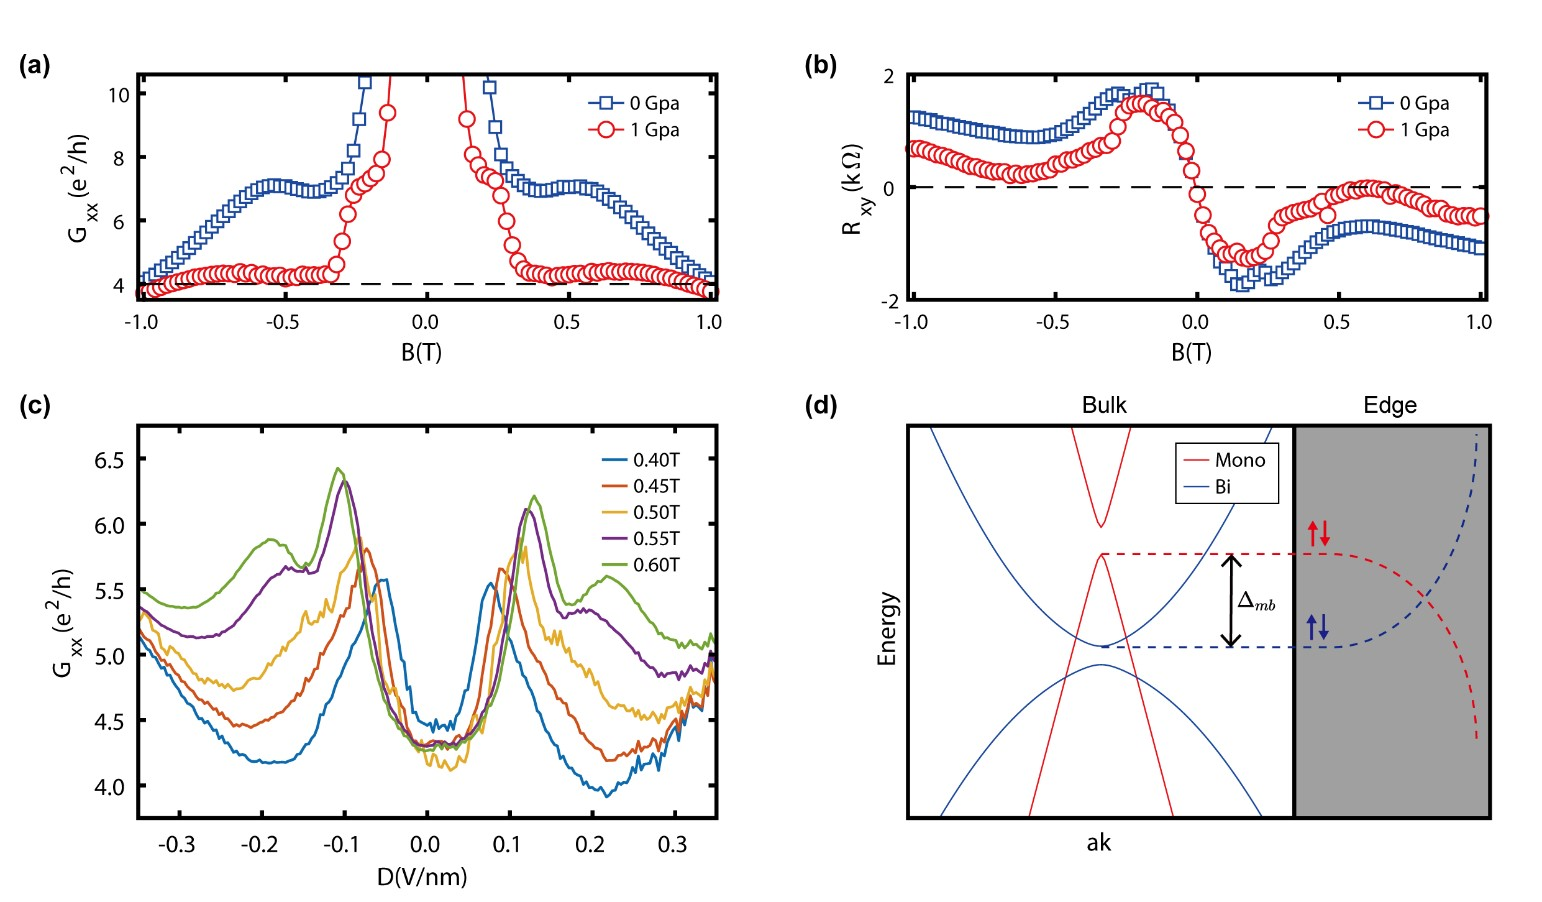
\includegraphics{figures/Figure_3.jpg}% Here is how to import EPS art
    \caption{\label{fig:3} Experimental signatures of Quantum Parity Hall effect and its schematics. \\
    (a) The longitudinal conductance $G_{xx}$ profiles of the D = 0 V/nm in both Figure~\ref{fig:2}(a) and ~\ref{fig:2}(b), blue squares mark the 0 GPa curve, 
    and red circles mark the 1 GPa curve. It can be seen that $G_{xx}$ becomes nearly quantized (about $4.1 \frac{e^2}{h}$) after pressure. 
    (b) The profiles of transverse resistance $R_{xx}$ at D = 0 V/nm, where the 1 GPa curve almost reaches zero around B = 0.6T, together with the nearly quantized signature in (a), 
    indicating the appearance of helical edge states in the system, which is the quantum parity hall state (QPHE). 
    (c) The profiles at B = 0.40 / 0.45 / 0.50 / 0.55 / 0.60 T are taken from Figure~\ref{fig:2}(b) as a function of displacement field D. The nearly quantized plateau disappears when D is large enough. 
    (d) The schematic of the mechanism of (QPHE) based on the band structure: the edge states from the monolayer valence band and that from the bilayer conduction band propagate along opposite directions 
    along the edge, and because of the spin degeneracy, there are four channels of edge states.
    }
\end{figure*}

% Table
\begin{table*}
\caption{\label{tab:table1}This is a table that records the fitting parameters at 0 Gpa and 1 Gpa based on the experimental results shown in figure.4(a)(b), \
the energy unit is set to $eV$. The intralayer hopping $\gamma_0$ is fixed as $3.100eV$.}
    \begin{ruledtabular}
        \begin{tabular}{ccccccccc}
            % &\multicolumn{2}{c}{$D_{4h}^1$}&\multicolumn{2}{c}{$D_{4h}^5$}\\
            Pressure & $\gamma_0$ & $\gamma_1$ & $\gamma_2$ & $\gamma_3$ & $\gamma_4$ & $\gamma_5$ & $\delta$ & $\Delta_2$ \\ \hline
            0 GPa & $3.100$ & $0.3845$ & $-0.0194$ & $0.3510$ & $0.0653$ & $0.0636$ & $0.0415$ & $0.0021$ \\
            1 GPa & $3.100$ & $0.3784$ & $-0.0234$ & $0.3665$ & $0.0612$ & $0.0833$ & $0.0534$ & $0.0031$ \\
        \end{tabular}
    \end{ruledtabular}
\end{table*}

\begin{figure*}
    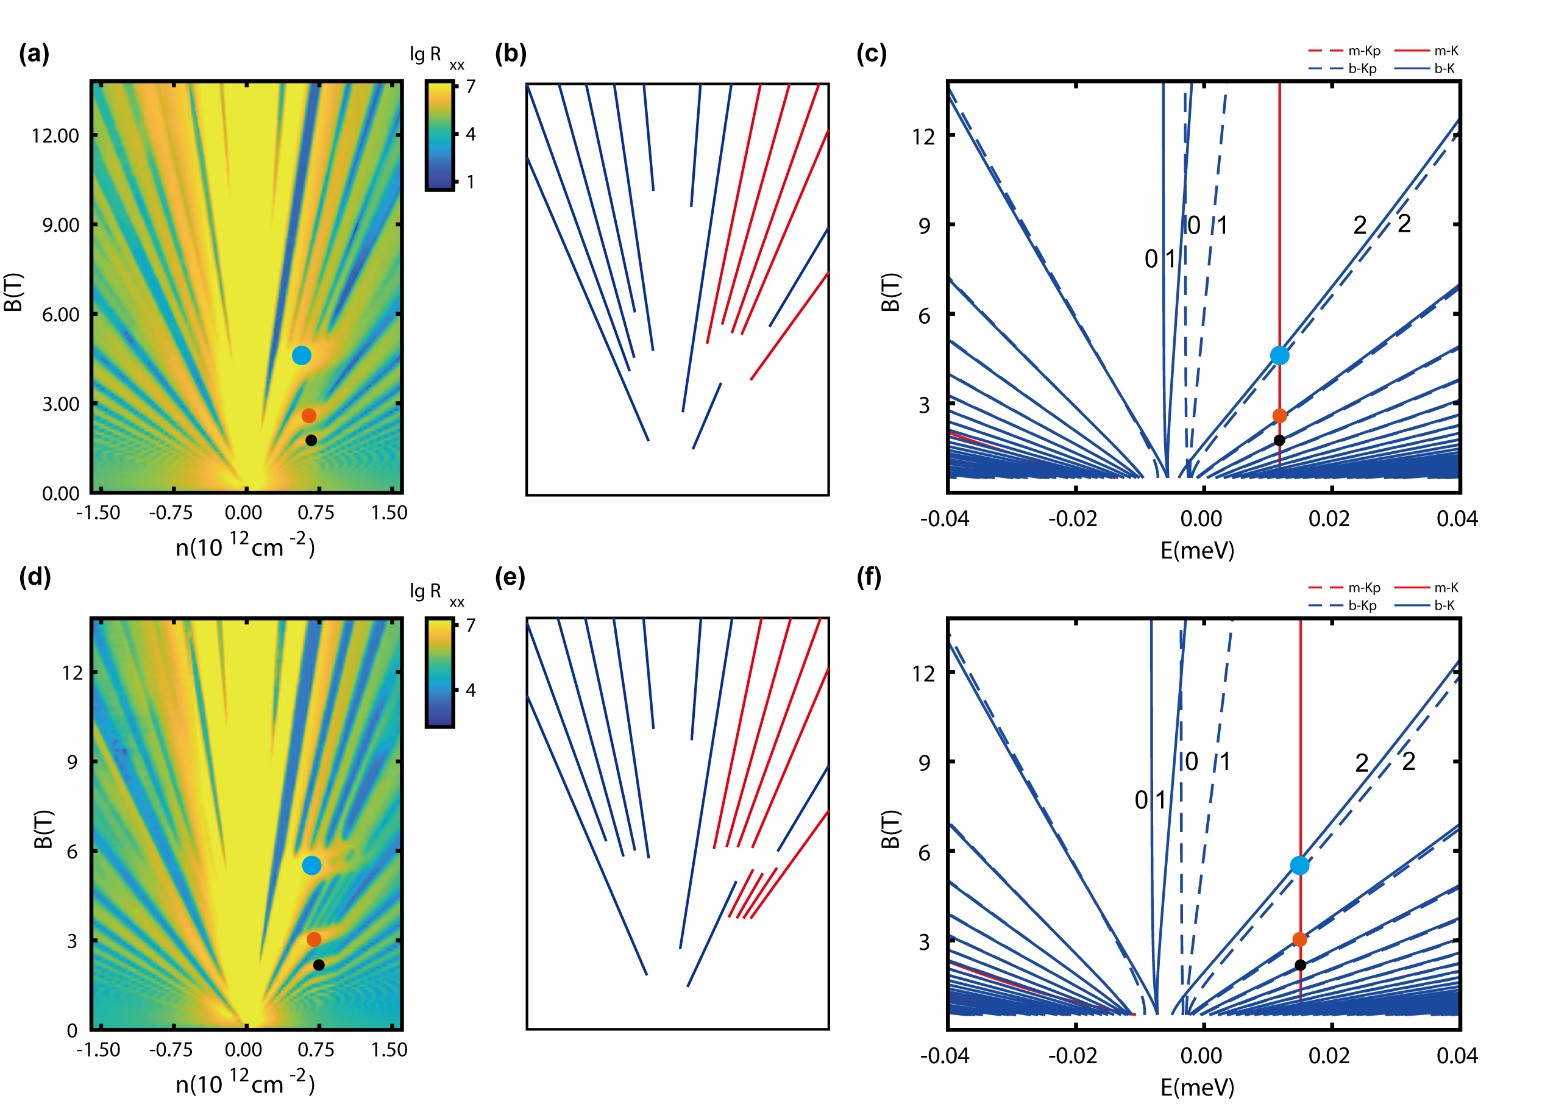
\includegraphics{figures/Figure_4.jpg}% Here is how to import EPS art
    \caption{\label{fig:4} Landau Fan diagrams at 0 GPa and 1 GPa, and the fitted simulation results.\\
    (a), (d) the Landau Fan diagrams at 0 GPa and 1 GPa, the crossing points between $(m, K/K^{\prime}, 0)$ and $(b, K^{\prime}, 2), (b, K^{\prime}, 3), 
    (b, K^{\prime}, 4)$ are marked by cyan, orange and black-coloured dots (P1, P2 and P3). It can be seen that the crossing points shift toward a large magnetic field 
    after pressure. In (b) (e), some minimum tracks at low integer fillings (from -6 to 10) are traced out, the blue colour indicates that the LLs are from a bilayer-like branch 
    while the red is from monolayer-like branch. (c), (f) the simulated Landau level structures fitted by the positions of crossing points from (a) and (b). 
    The corresponding points are also marked in the figures. The monolayer-like Landau levels are red-color, while the bilayer-like 
    Landau levels are blue-colour (dashed line for $K^{\prime}$ valley and solid line for $K$ valley). The numbers are the Landau level indexes in each branch. 
    The fitting parameters are listed in Table~\ref{tab:table1}.}
\end{figure*}